\documentclass[border=4pt]{standalone}

\usepackage{amsmath}
\usepackage{tikz}
\usepackage{mathdots}
\usepackage{yhmath}
\usepackage{cancel}
\usepackage{color}
\usepackage{siunitx}
\usepackage{array}
\usepackage{multirow}
\usepackage{amssymb}
\usepackage{gensymb}
\usepackage{tabularx}
\usepackage{booktabs}
\usetikzlibrary{fadings}
\usetikzlibrary{patterns}


\begin{document}
 


\tikzset{every picture/.style={line width=0.75pt}} %set default line width to 0.75pt        

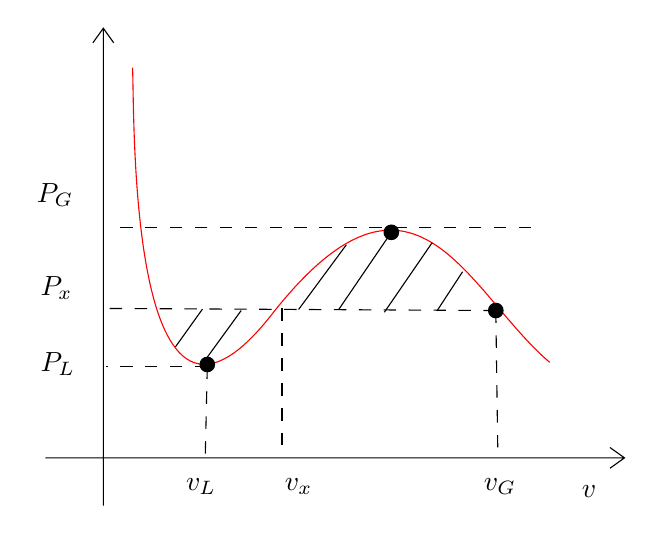
\begin{tikzpicture}[x=0.75pt,y=0.75pt,yscale=-1,xscale=1]
%uncomment if require: \path (0,300); %set diagram left start at 0, and has height of 300

%Shape: Axis 2D [id:dp07788990208156088] 
\draw  (72,238) -- (351,238)(99.9,31) -- (99.9,261) (344,233) -- (351,238) -- (344,243) (94.9,38) -- (99.9,31) -- (104.9,38)  ;
%Curve Lines [id:da6442275620961628] 
\draw [color={rgb, 255:red, 255; green, 0; blue, 0 }  ,draw opacity=1 ]   (114,50) .. controls (115,76) and (112,257) .. (181,169) .. controls (250,81) and (275,158) .. (315,192) ;


%Straight Lines [id:da584302188451362] 
\draw  [dash pattern={on 4.5pt off 4.5pt}]  (150,194) -- (149,238) ;


%Straight Lines [id:da5860801371383524] 
\draw  [dash pattern={on 4.5pt off 4.5pt}]  (289,167) -- (290,237) ;


%Straight Lines [id:da6588524919363896] 
\draw  [dash pattern={on 4.5pt off 4.5pt}]  (186,166) -- (186,236) ;


%Straight Lines [id:da39948858439820123] 
\draw  [dash pattern={on 4.5pt off 4.5pt}]  (150,194) -- (101,194) ;


%Straight Lines [id:da8372299377536021] 
\draw  [dash pattern={on 4.5pt off 4.5pt}]  (289,167) -- (99,166) ;


%Straight Lines [id:da6126502432898133] 
\draw  [dash pattern={on 4.5pt off 4.5pt}]  (306,127) -- (102,127) ;


%Shape: Circle [id:dp8746754942948474] 
\draw  [fill={rgb, 255:red, 0; green, 0; blue, 0 }  ,fill opacity=1 ] (146.5,193) .. controls (146.5,191.07) and (148.07,189.5) .. (150,189.5) .. controls (151.93,189.5) and (153.5,191.07) .. (153.5,193) .. controls (153.5,194.93) and (151.93,196.5) .. (150,196.5) .. controls (148.07,196.5) and (146.5,194.93) .. (146.5,193) -- cycle ;
%Straight Lines [id:da5971741178298731] 
\draw    (194,166.5) -- (217,135.33) ;


%Straight Lines [id:da9981917293274649] 
\draw    (213.33,166.5) -- (238.67,129.33) ;


%Straight Lines [id:da7533773310550331] 
\draw    (235.33,167.83) -- (258.33,134.33) ;


%Straight Lines [id:da7236135264155192] 
\draw    (260.67,167.17) -- (273,148.33) ;


%Straight Lines [id:da7459353708546717] 
\draw    (134.67,184.5) -- (147.67,166.33) ;


%Straight Lines [id:da972396014274783] 
\draw    (150,189.5) -- (166.33,167) ;


%Shape: Circle [id:dp07586442291095374] 
\draw  [fill={rgb, 255:red, 0; green, 0; blue, 0 }  ,fill opacity=1 ] (285.5,167) .. controls (285.5,165.07) and (287.07,163.5) .. (289,163.5) .. controls (290.93,163.5) and (292.5,165.07) .. (292.5,167) .. controls (292.5,168.93) and (290.93,170.5) .. (289,170.5) .. controls (287.07,170.5) and (285.5,168.93) .. (285.5,167) -- cycle ;
%Shape: Circle [id:dp4823881721047445] 
\draw  [fill={rgb, 255:red, 0; green, 0; blue, 0 }  ,fill opacity=1 ] (235.17,129.33) .. controls (235.17,127.4) and (236.73,125.83) .. (238.67,125.83) .. controls (240.6,125.83) and (242.17,127.4) .. (242.17,129.33) .. controls (242.17,131.27) and (240.6,132.83) .. (238.67,132.83) .. controls (236.73,132.83) and (235.17,131.27) .. (235.17,129.33) -- cycle ;

% Text Node
\draw (334,254) node    {$v$};
% Text Node
\draw (147,252) node    {$v_{L}$};
% Text Node
\draw (291,252) node    {$v_{G}$};
% Text Node
\draw (194,252) node    {$v_{x}$};
% Text Node
\draw (76.67,111.33) node    {$P_{G}$};
% Text Node
\draw (77.33,156) node    {$P_{x}$};
% Text Node
\draw (78,192.67) node    {$P_{L}$};


\end{tikzpicture}

\end{document}
